\documentclass[10pt, a4paper]{article}
\usepackage[utf8]{inputenc}
\usepackage{amsfonts}
\usepackage{amsmath}
\usepackage{amssymb}
\usepackage{amsthm}
\usepackage[all,cmtip]{xy}
\usepackage{hyperref}
\usepackage[top=3cm, left=3cm,right=3cm, bottom=3cm]{geometry}
\usepackage{graphicx}
%\usepackage{subfig}
%\usepackage{subfigure}
\usepackage{caption}
\usepackage{subcaption}
\usepackage{float}
\usepackage{tikzsymbols}
\usepackage{algorithm}
\usepackage{mathtools}
\usepackage[noend]{algpseudocode}
\newcommand{\E}[0]{\mathbb{E}}
\newcommand{\R}[0]{\mathbb{R}}
\newcommand{\Pp}[0]{\mathbb{P}}
\newcommand{\p}[0]{\mathfrak{p}}
\newcommand{\I}[0]{\mathcal{I}}
\newcommand{\F}[0]{\mathcal{F}}
\newcommand{\vv}[0]{\mathbf{v}}
\newtheorem{theorem}{Theorem}
\newtheorem{lemma}{Lemma}
\newtheorem{coro}{Corollary}
\newtheorem{definition}{Definition}
\theoremstyle{remark}
\newtheorem{rmk}{Remark}
\newtheorem{ex}{Example}




\title{Classification of functional fragments}
\author{William Borgeaud dit Avocat}
\date{}

\begin{document}
\maketitle
\subsection*{Full observations}
We perform classification on functional data using a quadratic discrimant analysis (QDA). We then try to generalize this method to the censored framework, where the data is not fully observed. \\
Our setup is as follows. We have two populations, $\Pi_0$ and $\Pi_1$, of functions in $\mathbb{L}^2[0,1]$ with means $\mu_i$ and covariance kernel $K_i$ for $i=0,1$. The kernels decompose as 
$$K_i(s,t) = \sum_{j = 0}^\infty \lambda_{ij} \phi_{ij}(s) \phi_{ij}(t) \text{ \ \ for } i=0,1.$$
The QDA classifier classifies a new observation $Y$ to population $\Pi_0$ if the test function
$$T(Y) = \sum_{j = 0}^{r} \left(\xi_{0j}^2-\xi_{1j}^2 + \log \frac{\lambda_{0j}}{\lambda_{1j}}\right) < 0,$$
where the $\xi_{ij}$ are the standardized random variables in the KL expansion of $X \sim \Pi_i$:
$$X-\mu_i = \sum_{j=0}^{\infty} \sqrt{\lambda_{ij}}\xi_{ij} \phi_{ij} \text{ \ \ for } i=0,1.$$
In practice, we observe curves $X_{ik} \sim \Pi_i$, $i=0,1$, $k=1,...,n_{i}$ on the grid $\{0,\frac{1}{N}, ..., \frac{N-1}{N},1\}$ and we estimate $\mu_i, K_i$ by the usual sample estimates $\hat{\mu}_i, \hat{K}_i$, from which we get estimates $\hat{\lambda}_{ij}$, $\hat{\phi}_{ij}$, $\hat{\xi}_{ij}$. From these, given a new observation $Y$, we can compute the empirical version of the test function 
\begin{equation}\label{test}
	\hat{T}(Y) = \sum_{j = 0}^{rk(\hat{K})} \left(\hat{\xi}_{0j}^2-\hat{\xi}_{1j}^2 + \log \frac{\hat{\lambda}_{0j}}{\hat{\lambda}_{1j}}\right)
\end{equation}
and use it to classify $Y$ to population $\Pi_0$ if $\hat{T}(Y)<0$ and to $\Pi_1$ otherwise.

\subsection*{Censored observations}
When the curves are not fully observed, we adapt the QDA classifier in the following way. We compute the estimators $\tilde{\mu}_i$, $\tilde{K}_i$, $i=0,1$ using the methods described in \cite{pana}. Then given a new observation $Y$ defined on a subinterval $\mathcal{J} \subseteq [0,1]$, we use the test function $T$ as in \ref{test}, but with all values restricted to $\mathcal{J}$. More precisely, we compute the estimates $\hat{\lambda}_{ij}$, $\hat{\phi}_{ij}$, $\hat{\xi}_{ij}$ using $(\tilde{\mu}_i)|_\mathcal{J}$ and $(\tilde{K}_i)|_{\mathcal{J} \times \mathcal{J}}$.

\subsection*{Numerical experiments}
We consider three bases of $\mathbb{L}^2[0,1]$:
\begin{itemize}
	\item $B_1 = \{\phi_0(t)=1, \phi_n(t)= \sqrt{2}\cos(2n\pi t)\}$,
	\item $B_2 = \{\phi_0(t)=1, \phi_n(t)= \sqrt{2}\sin(2n\pi t)\}$,
	\item $B_3 =$ Legendre polynomials basis.
\end{itemize}
For each experiments, we generate $n=200$ samples from each population $\Pi_0$ and $\Pi_1$ on a regular grid of size $N=100$. 

\subsubsection*{Observation: Reducing the rank increases accuracy}
We use the basis $B1$ and the mean $\mu = 0$ for both populations. The difference lies in the $\lambda$'s:
$$\vec{\lambda}_0 = (1.5,0.5,0.1,0.05,|z_1|,...,|z_{16}|), \ \vec{\lambda}_1 = \vec{\lambda}_0 + 1, \ z_i \sim \mathcal{N}\left(0,\frac{1}{1000}\right),$$
so that population $\Pi_1$ varies a lot more around its mean, see Figure \ref{fig:samples}. 
\begin{figure}[h]
\centering
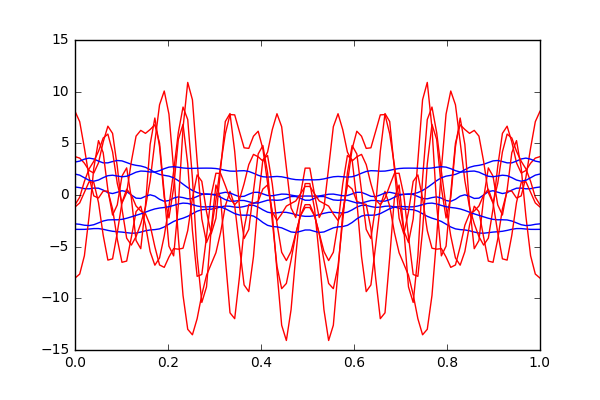
\includegraphics[width=0.7\linewidth]{Code/report_images/samples}
\caption{Blue: $\Pi_0$, Red:$\Pi_1$.}
\label{fig:samples}
\end{figure}\\
Using the QDA classifier, we (surprisingly) get a training accuracy of 100\% for $\Pi_0$ and of 0\% for $\Pi_1$ and the same result for the testing accuracy. However, by reducing the rank of $\hat{K}_i$ using SVD, we can get perfect classification, both in training and testing, see Figure \ref{fig:accu-rank}.
\begin{figure}[h]
\centering
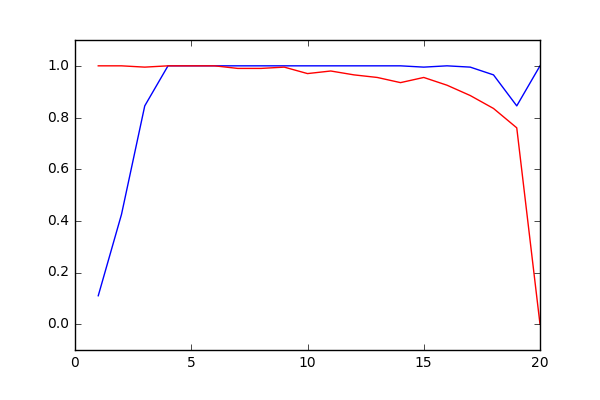
\includegraphics[width=0.7\linewidth]{Code/report_images/accu-rank}
\caption{Training accuracy of the classifier depending on the rank of $\hat{K}_i$}
\label{fig:accu-rank}
\end{figure}
\textbf{Why?}

\subsubsection*{Observation: The covariance estimation from fragments can yield a bad accuracy}
We use basis $B_2$ for both population, $\mu_0=0$, $\mu_1(t)=\frac{1}{2} + t$, $\vec{\lambda}_0$ as in the previous experiment and $\vec{\lambda}_1$ a slight deviation of $\vec{\lambda}_0$. When observing the full curves, we get relative errors of $0.10$ and  $0.18$ for $\hat{K}_0$ and $\hat{K}_1$, and when we observe fragments with $\delta=0.9$, we get $0.11$ and $0.20$, see Figure \ref{fig:covs}. 
\begin{figure}
\centering
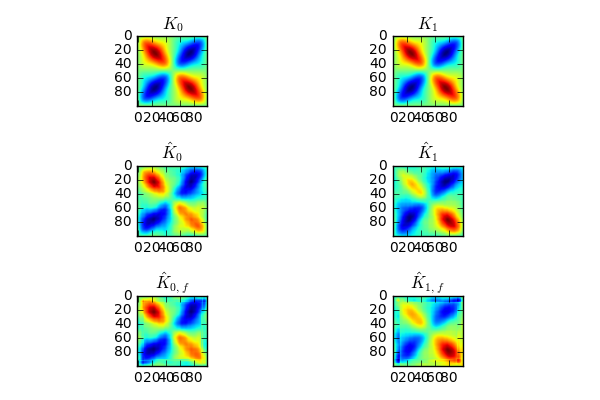
\includegraphics[width=0.7\linewidth]{Code/report_images/covs}
\caption{Heat maps of covariance kernels}
\label{fig:covs}
\end{figure}\\
Thus the covariance estimation is not all that worse when observing fragments. However, when performing classification, we get perfect training and testing accuracy scores for both populations with the full curves, but with the fragments, we get accuracy scores of $0.75, 0.73$ for training and of $0.70, 0.68$ for testing. Moreover, the problem does not lie in the observation of fragments but in the estimation of the covariance. Indeed, when using $\tilde{K}_i$ in the full curves classifier, we get similar error rates. Conversely, when using $\hat{K}_i$ in the fragments classifier we get bear-perfect accuracy. \textbf{Why?}

\subsubsection*{Experiment on fragments}
We use basis $B_3$ and $B_2$ for populations $\Pi_0$ and $Pi_1$ with the same $\vec{\lambda}_i$ as in the previous experiment, $\mu_0 = 0$, $\mu_1(t)=t$. For this experiment, we use $N=50$ to speed up the computations. Examples of fragments with $\delta = 0.5$ are shown in Figure \ref{fig:fragex}.
\begin{figure}
\centering
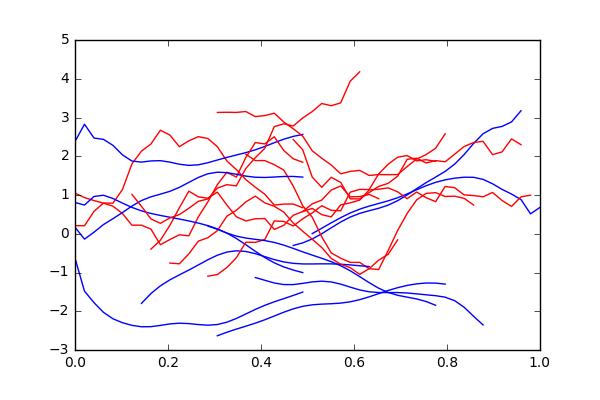
\includegraphics[width=0.7\linewidth]{Code/report_images/fragex}
\caption{10 fragments of curves from each population with $\delta=0.5$.}
\label{fig:fragex}
\end{figure}

We perform the classification task 20 times on these populations either with $\delta=0.1,0.2,...,0.9$, using a rank reduction, as in the first experiment, or with the full curves classifier. The plots of the medians of the relative errors for the covariance estimation are shown in Figure \ref{fig:coverr}, the errors for $\Pi_0$ in Figure \ref{fig:err1}, and the errors for $\Pi_1$ in Figure \ref{fig:err2}. These results all seem pretty natural. It is interesting to note that the relative errors for the covariance estimations seems to decrease at an exponential rate as $\delta$ increases. Also, it seems like there is a substantial increase in accuracy between $\delta=0.5$ and $\delta=0.6$ for both populations. We will investigate this further.
\begin{figure}[h]
\centering
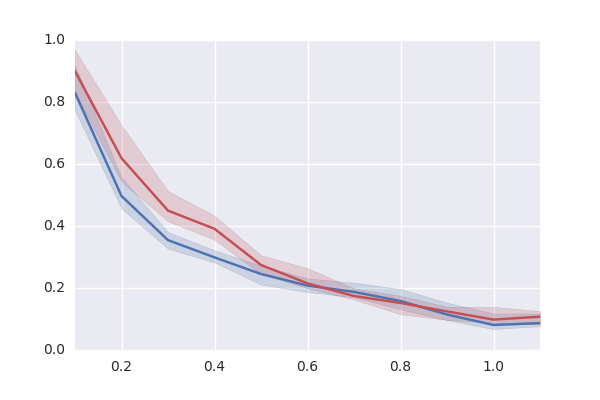
\includegraphics[width=0.7\linewidth]{Code/report_images/coverr}
\caption{Relative errors for the covariance estimations, with 95\% quantile bands. (1.1 value is with full curves.)}
\label{fig:coverr}
\end{figure}
\begin{figure}
\centering
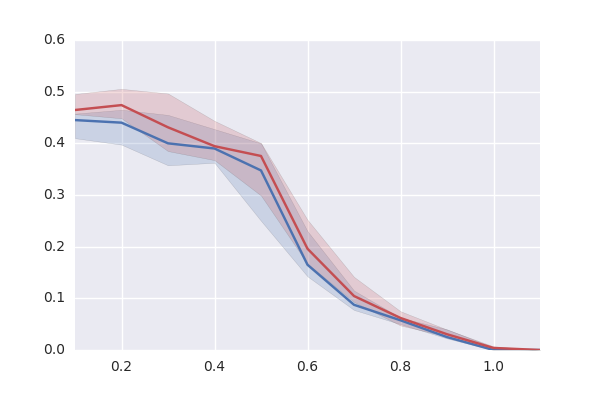
\includegraphics[width=0.7\linewidth]{Code/report_images/err1}
\caption{Training (blue) and testing (red) errors for population $\Pi_1$. (1.1 value is with full curves.)}
\label{fig:err1}
\end{figure}
\begin{figure}
\centering
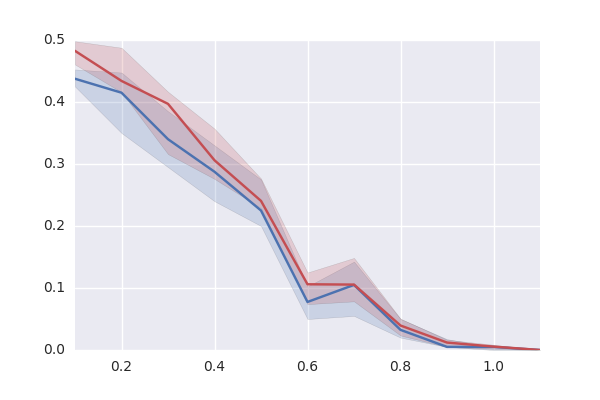
\includegraphics[width=0.7\linewidth]{Code/report_images/err2}
\caption{Training (blue) and testing (red) errors for population $\Pi_0$. (1.1 value is with full curves.)}
\label{fig:err2}
\end{figure}\\

\subsubsection*{Observation: Need to sum on $N$ not $r$}



\begin{thebibliography}{1}
	
	\bibitem{pana} Marie-Hélène Descary, Victor M. Panaretos {\em Recovering Covariance from Functional Fragments}  2017	.
	
\end{thebibliography}


\end{document}